\documentclass[utf8]{gradu3}
% Jos työ on kandidaatintutkielma eikä pro gradu, käytä ylläolevan asemesta
%\documentclass[utf8,bachelor]{gradu3}
% Jos kirjoitat englanniksi, käytä ylläolevan asemesta
%\documentclass[utf8,english]{gradu3}
% tai
%\documentclass[utf8,bachelor,english]{gradu3}

\usepackage{graphicx} % kuvien mukaan ottamista varten

\usepackage{amsmath} % hyödyllinen jos tekstisi sisältää matikkaa,
                     % ei pakollinen

\usepackage{booktabs} % hyvä kauniiden taulukoiden tekemiseen
\usepackage{listings}
\usepackage{color}
\usepackage{qtree}

% HUOM! Tämän tulee olla viimeinen \usepackage koko dokumentissa!
\usepackage[bookmarksopen,bookmarksnumbered,linktocpage]{hyperref}

\addbibresource{thesis.bib} % Lähdetietokannan tiedostonimi

\definecolor{light-gray}{gray}{0.96}

\lstdefinelanguage{Smalltalk}{
morekeywords={true,false,self,super,nil},
sensitive=true,
morecomment=[s][\color{blue}]{"}{"},
morestring=[d]',
alsoother={_},
style=SmalltalkStyle,
columns=fullflexible,
backgroundcolor=\color{light-gray},
xleftmargin=.20in,
showspaces=false,
numbers=left,
framexleftmargin=15pt,
tabsize=4
}
\lstdefinestyle{SmalltalkStyle}{
literate={:=}{{$\gets\ $}}2{^}{{$\uparrow$}}1{_}{{$\gets\ $}}2{ä}{{\"a}}2{ö}{{\"o}}2
}


\begin{document}

\title{\LaTeX-tutkielmapohjan {gradu3} käyttö}
\translatedtitle{Usage of the {gradu3} document class for \LaTeX\ theses}
\studyline{Kaikki suuntautumisvaihtoehdot}
\avainsanat{%
  \LaTeX,
  {gradu3},
  pro gradu -tutkielmat,
  kandidaatintutkielmat,
  käyttöohje}
\keywords{\LaTeX, {gradu3}, Master's Theses, Bachelor's Theses, user's guide}
\tiivistelma{%
  Tämä kirjoitelma on esimerkki siitä, kuinka
  {gradu3}-tutkielmapohjaa käytetään.  Se sisältää myös
  käyttöohjeet ja tutkielman rakennetta koskevia ohjeita.

  Tutkielman tiivistelmä on tyypillisesti lyhyt esitys, jossa
  kerrotaan tutkielman taustoista, tavoitteesta, tutkimusmenetelmistä,
  saavutetuista tuloksista, tulosten tulkinnasta ja johtopäätöksistä.
  Tiivistelmän tulee olla niin lyhyt, että se, englanninkielinen
  abstrakti ja muut metatiedot mahtuvat kaikki samalle sivulle.
}
\abstract{%
  This document is a sample {gradu3} thesis document class
  document.  It also functions as a user manual and supplies
  guidelines for structuring a thesis document.

  The English abstract of a thesis should usually say exactly the same
  things as the Finnish tiivistelmä.
}

\author{Antti-Juhani Kaijanaho}
\contactinformation{Ag~C416.1, \texttt{antti-juhani.kaijanaho@jyu.fi}}
% jos useita tekijöitä, anna useampi \author-komento
\supervisor{Ohjaamaton työ}
% jos useita ohjaajia, anna useampi \supervisor-komento

\type{tutkielmapohjan esimerkki ja käsikirja} % et tarvitse tätä riviä tutkielmassa!

\maketitle

\preface
Tähän voit kirjoittaa tutkielmasi esipuheen.  Tutkielmissa on
harvemmin esipuheita, mutta jos sen kirjoitat, pidä se lyhyenä
(enintään sivu).

Esipuheen tulisi kertoa ennemminkin tutkielmaprosessista kuin
tutkielman sisällöstä.  Esimerkiksi jos tutkielman aiheen valintaan
tai tekemiseen liittyy jokin erikoinen sattumus, voit siitä kertoa
esipuheessa.  Tapana esipuheessa on myös kiittää nimeltä mainiten
tärkeimpiä tutkielman tekemisessä auttaneita ihmisiä -- ainakin
ohjaajia, puolisoa ja lapsia.  (Yleensä perhe on auttanut vähintään
tukemalla ja kannustamalla.)

Esipuhe kannattaa kirjoittaa minä-muodossa. Tavanomaista on myös
allekirjoittaa se.

Jyväskylässä \today

\bigskip

Tutkielman tekijä


\begin{thetermlist}
\item[Sovellusarkkitehtuuri] Donald Knuthin 1977--1989 laatima eräajotyyppinen
  ladontajärjestelmä \parencite[ks.][]{knuth86:_texbook}. 
\item[MVC] \TeX in \parencite[ks.][]{knuth86:_texbook} päälle
  rakennettu rakenteisten kirjoitelmien ladontaan tarkoitettu
  järjestelmä \parencite[ks.][]{lamport94:_latex}.  Siitä on nykyään
  käytössä versio \LaTeXe.
\item[Sovelluskehys] \TeX in \parencite[ks.][]{knuth86:_texbook} päälle
  rakennettu rakenteisten kirjoitelmien ladontaan tarkoitettu
  järjestelmä \parencite[ks.][]{lamport94:_latex}.  Siitä on nykyään
  käytössä versio \LaTeXe.
\end{thetermlist}

\chapter{Johdanto}

\section{Tausta}
\section{Tutkimuskysymys}
MVC-arkkitehtuuri on saanut paljon huomiota web-sovelluskehyksien
toteutuksissa ja useat web-sovelluskehykset ovat luokiteltu
MVC-pohjaisiksi sovelluskehyksiksi \parencite{mvcframeworks}. Se on kuitenkin alunperin
tarkoitettu matalan tason käyttöliittymäsovellusten toteuttamiseen,
jossa esimerkiksi hallitaan yksittäisiä näppäimistöltä tulleita
syötteitä eikä sitä ole suoraan tarkoitettu käytettäväksi
web-sovellusten ohjelmointiin. Alkuperäisen MVC:n toteutuksen
soveltuvuutta web-ohjelmointiin onkin epäilty. Esimerkiksi Leff
soveltaa artikkelissaan MVC:n käyttämistä web-sovelluksissa, mutta
samalla esittelee alkuperäisen MVC:n toteuttamisen ongelmana. Tämä johtuu web-sovelluksen jakautumisesta asiakkaan
(client) ja palvelimen (server) välille \parencite{ibm_watson}. Myös Pyramid-sovelluskehyksen tekijät
kyseenalaistavat MVC-arkkitehtuurin toteutuksen Pyramidissa ja uskovat
MVC:n olevan sellaisenaan sopimaton web-ohjelmointiin, vaikka
Pyramidin toteutus onkin hyvin lähellä alkuperäistä MVC:tä
\parencite{pyramid}. Django on myös toteutettu MVC:n pohjalta, mutta
se ei kuitenkaan toteuta MVC:tä sellaisenaan \parencite{django}.

Tutkimuksen tarkoituksena on selvittää millä tavalla
MVC-arkkitehtuuri on toteutettu web-sovelluskehyksissä ja miten se
eroaa alkuperäisestä MVC:n toteutuksesta. Lisäksi laajennetaan
Flask-sovelluskehys toteuttamaan alkuperäinen MVC niinkuin Krasner on
sen määritellyt \parencite{krasner}. Havaintojen pohjalta
selvitetään voidaanko MVC tuoda sellaisenaan sovelluskehykseen ja
mitä mahdollisia ongelmia se tuo.

\chapter{Oletus}
Tässä oletetaan mitä tutkimuskysymykseen voisi tulla vastaukseksi

\chapter{Tutkimuksen Rakenne}
Tutkimus aloitetaan kirjallisuuskatsauksella, jossa tarkastellaan mitä aiempaa 
tutkimusta MVC:stä on tehty. Lisäksi käydään
läpi mitä lähteitä löytyy Python-pohjaisista web-sovelluskehyksistä. Tämän jälkeen 
tutkitaan MVC:n historiaa sekä millä tavalla MVC on tarkoitettu toteutettavaksi.
Tässä vaiheessa käydään läpi jokaisen MVC-komponentin tarkoitus sekä niiden 
keskinäisen kommunikaation rakentuminen. Lisäksi esitellään
Dortmundin yliopistossa kirjoitettu esimerkkiohjelma Smalltalkilla siitä miten MVC:n 
toteutus tuodaan sovellukseen käytännössä.

MVC:n tarkastelun jälkeen esitellään tutkimuksessa käytetyt web-sovelluskehykset, 
joita käytetään apuna MVC:n tutkimisessa. Sovelluskehyksistä käydään läpi sen 
historia sekä yleisellä tasolla mihin käyttötarkoitukseen
sovelluskehys on tarkoitettu. Tämän jälkeen verrataan MVC:n toteutusta erikseen 
jokaiseen sovelluskehykseen ja selvitetään millä tavalla niiden sovellusarkkitehtuuri 
mahdollisesti eroaa MVC:stä,
Havaintojen perusteella pohditaan MVC:n mahdollisia ongelmia sovelluskehyksien toteutuksessa 
ja selvitetään löytyykö sovelluskehyksien arkkitehtuurista jotain yhtenäisiä piirteitä, mitkä ovat
kytköksissä MVC:n toteutukseen. Saatujen tulosten pohjalta  kirjoitetaan Flask-sovellus, joka toteuttaa MVC:n 
niinkuin se on alunperin tarkoitettu.

Tutkimuksen lopuksi koostetaan havainnoista yhteenveto, jossa pohditaan saatuja tuloksia ja selvitetään 
pystytäänkö niiden perusteella vastaamaan tutkimuskysymykseen.


\section{Aiheen rajaus}
Tutkimus on rajattu tarkastelemaan MVC-arkkitehtuurin
toteutusta Pythonilla kirjoitetuissa
web-sovelluskehyksissä. Tarkasteltavat web-sovelluskehykset rajataan 
Pyramid-, Django-, Plone- sekä Flask-sovelluskehyksiin. Pyramid, Django ja Plone toteuttavat MVC:n kaltaisen
sovellusarkkitehtuurin. Flask on sovelluskehys, joka tarjoaa vain
välttämättömät kirjastot web-sovelluksen toteuttamiseen. Sitä
käytetään tutkimuksessa työkaluna selvittämään miten MVC tulisi
toteuttaa sovelluskehykseen. MVC:stä on olemassa erilaisia versioita, joten sen määrittely tulee rajata tarkasti.
Kun puhutaan MVC:stä tarkoitetaan tällä Krasnerin
artikkelissa esiteltyjä määrittelyitä MVC:n
toteutuksesta \parencite{krasner}, jotka pohjautuvat Trygve Reenskaugin esittelemään 
MVC:n määritelmään \parencite{xerox-original}. 

Tarkasteltavat sovelluskehykset käydään ensiksi yleisellä tasolla läpi, jonka jälkeen niitä tarkastellaan MVC:n näkökulmasta. Yleisellä tasolla tarkoitetaan sovelluskehyksen historian ja käyttötarkoituksen esittelemistä. Sovelluskehyksien muihin teknisiin ominaisuuksiin ei oteta kantaa. Flask-osiossa MVC-arkkitehtuuri toteutaan niinkuin se on Krasnerin julkaisussa määritelty. Näiden havaintojen pohjalta pyritään vastamaan tutkimuskysymykseen.


\chapter{Kirjallisuuskatsaus}
\section{Toteutus}
Kirjallisuuskatsauksessa käydään läpi vaihe vaiheelta, miten
lähdemateriaalia kerätään tutkimusta varten. Lähdemateriaalin 
haku toteutetaan hakukoneilla, jotka ovat tarkoitettu erityisesti 
tieteellisten artikkeleiden etsimiseen. Tässä tutkielmassa käytetyt 
hakukoneet ovat seuraavat: IEEE Xplore, ACM Digital Library, 
Google Scholar sekä joissakin tapauksissa Google:n yleinen
hakukone. Yleistä hakukonetta on käytetty esimerkiksi
sovelluskehyksien dokumentaatioiden etsintään.

Aluksi muodostetaan kokonaiskuva tuloksista, jolloin silmäillään läpi
saatuja artikkeleita. Tässä vaiheessa tarkoitus ei ole vielä valita
mitään pohjaksi tutkielmalle, vaan kerätä informaatiota siitä
millainen lähdemateriaali on tarjolla kokonaisuudessaan. Saaduista 
tuloksista poimitaan artikkeleita, jotka sopivat tutkimuksen aihepiiriin.
Seuraavaksi artikkeleista valitaan tutkielmalle
pohjakirjallisuus. Tässä vaiheessa artikkelit luetaan huolellisesti
läpi ja varmistutaan siitä, että ne ovat tieteellisesti päteviä
tutkielmaa varten. Erityisesti kiinnitetään huomiota viittauksien
määrän valittaessa tärkeimmät lähdemateriaalit. Tutkielmassa esiintyy myös satunnaisia viittauksia,
joita ei ole kirjallisuuskatsauksessa mainittu. Tutkimuksen
pääkirjallisuus kuitenkin käydään läpi kirjallisuuskatsauksessa.
Haussa käytetään seuraavia hakutermejä: "MVC", "MVC Architecture",
"frameworks", "web frameworks" ja  "MVC- Architecture". Erityisesti artikkeleita löytyy
MVC-arkkitehtuurin soveltamisesta erilaisissa
tekniikoissa. Tarkasteltavat artikkelit rajataan kuitenkin niihin,
jotka esittelevät suoraan MVC:tä itseään tai tarjoavat
lähdemateriaalin sovelluskehyksien esittelyyn.

\section{MVC}
Google Scholarin tuloksista löytyy kolme artikkelia MVC:stä, jotka sopivat 
lähdemateriaaliksi tutkimukseen. Ensimmäinen artikkeleista on John
Deaconin  kirjoittama artikkeli, joka tarkastelee lyhyesti
MVC:tä \parencite{deacon}. Artikkeli on kuitenkin hyvin suppea, mutta selittää
tiivistetysti MVC:n idean. Toinen artikkeli on Steve Burbeckin kirjoittama, 
joka käsittelee
MVC:tä sellaisena kuin sitä käytettiin Smalltalkissa \parencite{burbeck}. Burbeckin
artikkeliin viitataan monissa MVC:tä käsittelevissä
julkaisuissa, joten sen arvo tämän tutkielman pohjakirjallisuudessa on
vahva. Viittausten määrä on katsottu hakemalla artikkelia Google
Scholarin hakukoneessa. Viittauksia kyseiseen artikkeliin on
kirjoitushetkellä 308. Seuraavaksi kartoitetaan pohjakirjallisuutta käyttäen ACM Digital
Library sekä IEEE XPlore -hakukoneita. Kolmas artikkeli Glenn
E. Krasnerin kirjoittama julkaisu, jossa esitellään MVC:n toteutusta
erilaisissa Smalltalk-sovelluksissa. Julkaisusta löytyy useita
versioita, joista tässä tutkielmassa käytetään
molempia \parencite{krasner} \parencite[krasner_desc]. Tähän artikkeliin on
myös viitattu runsaasti, joten se on Burbeckin julkaisun kanssa
tärkeimpiä lähteitä MVC:n pohjakirjallisuudessa. Kirjoitushetkellä
viittauksia Krasnerin artikkeliin on 2263. Monien MVC-arkkitehtuuria soveltavien artikkeleiden
lähdeviitteistä löytyy viittauksia Burbeckin ja Krasnerin
artikkeleihin. Tämän perusteella pystytään toteamaan kyseisten
artikkeleiden olevan tieteellisesti päteviä ja tarjoavan kattavan
lähdemateriaalin MVC:n pohjaksi. Burbeckin ja Krasnerin kirjoittamien
artikkeleiden taustalta löytyy MVC-arkkitehtuurin alkuperäinen kehittäjä Trygve
Reenskaug, jonka omia julkaisuja sekä kotisivujen MVC-osiota käytetään
myös lähteenä tutkielmassa \parencite{xerox}. Erityisesti Reenskaugin ja Adele Goldbergin
julkaisu, jossa kerrotaan jokaisen MVC komponentin tehtävä....


\section{Web-sovelluskehykset}
Web-sovelluskehyksistä löydetty kirjallisuus on hyvin
suppea, eikä niiden varaan voida rakentaa kovinkaan perusteellista
tieteellistä pohjaa. Tämän vuoksi tutkimuksessa joudutaan osaksi turvautumaan
sovelluskehyksien omaan dokumentatioon täydentämään
lähdemateriaalia. IEEE Xploren ja ACM Digital Libraryn avulla löytyy kolme julkaisua, 
joita käytetään tutkimuksen pohjana sovelluskehyksiä
tarkastellessa. Ensimmäinen artikkeli on Okanovicin ja Mateljan
kirjoittama artikkeli, jossa esitellään web-sovelluskehyksien suunnittelua \parencite{ockanovic}. 
Se myös sivuuttaa lyhyesti MVC:tä. Toisena artikkelina käytetään ACM:stä tuloksena saatua Iwan
Vosloon julkaisua, jossa käydään läpi yleisesti web-sovelluskehyksien
rakennetta \parencite{vosloo}. Kolmanneksi hyödynnetään Ignacion artikkelia, jossa esitellään ketteriä
web-sovelluskehyksiä sekä millä tavalla näitä tulisi vertailla \parencite{ignacio}.

Google Scholarin hakutuloksista löytyi Liza Daly:n
kirjoittama ja O'Reillyn julkaisema "Next Generation Web Frameworks
in Python", joka sisältönsä puolesta sopii hyvin pohjaksi
tutkimuksessa käsiteltävien sovelluskehyksien lähdemateriaaliksi 
\parencite{liza}.

\chapter{MVC}
MVC-arkkitehtuurin perusajatus on erottaa käyttöliittymä sovelluslogiikasta ja
näin tehdä sovelluksesta helposti ylläpidettävä kolmen eri komponentin avulla:
Malli (Model), Näkymä (View) ja Ohjain (Controller). Jokainen komponentti on
erikoistunut sovelluksessa johonkin tiettyyn tehtävään. Mallin tehtävänä on
hallita sovelluksen tilaa ja vastata sen käsittelemästä datasta ohjaimelle ja näkymälle.
Näkymän tehtävänä on taas näyttää sovelluksen käyttöliittymä ja sitä kautta mallin dataa. 
Ohjaimen tarkoitus on ottaa vastaan syötteitä käyttäjältä käskien mallia ja näkymää muuttumaan tarvittaessa.

\begin{figure}[h]
\centering
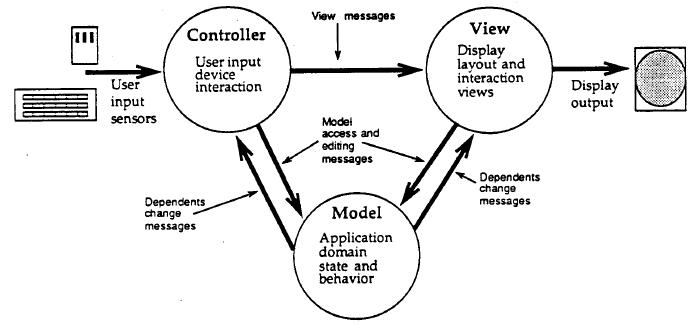
\includegraphics[scale=0.85]{krasner_mvc.jpg}
\caption{Model-View-Controller State and Message Sending \cite[s. 5]{krasner_desc}}
\end{figure} 
Jokaisella komponentilla on oma rajattu tehtävänsä ja ohjelmakoodi tulee jakaa näiden komponentien kesken. Jotta MVC:tä pystyttäisiin käyttämään
tehokkaasti, tulee ymmärtää komponenttien työnjako sekä se kuinka komponentit kommunikoivat keskenään \parencite{burbeck}. 

Luodessamme MVC-arkkitehtuurin toteuttavia komponentteja, tulee ne periä jostakin abstraktista pohjaluokasta (Model, View tai Controller), joka määrittelee kyseisen komponentin käyttäytymisen MVC:ssä  \parencite[s. 5]{krasner_desc}.  Tässä kappaleessa käydään jokaisen komponentin toteutus erikseen läpi käyttäen ohjelmointikielenä Smalltalkia. Lähteenä käytetään Krasnerin julkaisua \parencite{krasner_desc}.

Yleisesti MVC-komponenttien toimintaa kuvaavassa esimerkissä käyttäjältä tulee jokin syöte, jonka sillä hetkellä aktiivinen ohjain ottaa vastaan. Syötteen perusteella ohjain lähettää mallille viestin. Malli puolestaan tekee sille määrättyjä operaatioita muuttaen tilaansa ja lähettää edelleen viestin muutoksestaan kaikille siihen liitetyille riippuvuuksille (näkymät ja ohjaimet). Näkymät
voivat tämän jälkeen kysyä mallilta sen nykyistä tilaa ja päivittää itsensä, jos siihen on tarvetta. Ohjaimet voivat myös muuttaa tilaansa riippuen mallin tilasta \parencite[s. 4]{krasner_desc}. 

Suurin merkitys MVC:llä on luoda silta ihmismielen hahmottamalle mallille ja tietokoneessa esiintyvälle mallille. Oikein toteutettuna MVC:n avulla luodaan illuusio siitä, että käyttäjä kommunikoi suoraan mallin kanssa. Todellisuudessa kuitenkin ohjain ja näkymä muodostavat yhdessä rajapinnan sille, miltä malli näyttää ulospäin ja miten sitä käsitellään. Ohjain huolehtii syötteiden vastaanottamisesta ja käsittelemisestä. Näkymä taas huolehtii mallin graafisesta puolesta \parencite[s. 11-12]{reenskaug_tools}. 

\section{Historia}
MVC:n esitteli Norjalainen Trygve Reenskaug ollessaan mukana Xerox PARC -tutkimushankkeessa. 
Ensimmäinen julkaisu MVC:stä kirjoitettiin vuonna 1978 samassa tutkimuskeskuksessa. 
Tuolloin julkaisussa esiteltiin kolmen komponentin sijasta neljä komponenttia: 
Malli (Model), Näkymä(View), Ohjain(Controller) sekä Muokkaaja(Editor). Muokkaaja on 
väliaikainen komponentti, jonka näkymä luo itsensä ja syötelaitteiden välille. 
Muokkaaja-komponentista kuitenkin luovuttiin käsitteenä ja se sisällytettiin näkymään 
ja ohjaimeen \parencite{xerox}. Alkuperäinen Xerox PARC:n tuottama raportti MVC:stä oli Reenskaugin 
vuonna 1979 kirjoittama THING-MODEL-VIEW-EDITOR \parencite{xerox-thing}. Raportti esitteli MVC:n 
komponentteja käyttäen hyväksi esimerkkejä Reenskaugin omasta suunnittelutyöstä. Thing-komponentilla mallinnettiin
jotakin isompaa kokonaisuutta, joka hallitsee pienempiä kokonaisuuksia. Sitä voidaan ajatella eräänlaisena suurena mallina,joka on jaettu useisiin pienempiin malleihin. Editor-komponentti luo rajapinnan käyttäjän ja yhden tai useamman näkymän välille. Se tarjoaa käyttäjälle sopivan komento-rajapinnan kuten esimerkisi valikon, joka vaihtuu sisällön muuttuessa \parencite{xerox-thing}. Reenskaug hylkäsi kuitenkin Editor- ja Thing-komponentin ja  päätyi Adele Goldbergin avustuksella termeihin Models-Views-Controllers julkaisten saman vuoden lopulla raportin, jossa määritellään lyhyesti jokaisen komponentin tehtävä (MODELS-VIEWS-CONTROLLERS) \parencite{xerox-original}. Koska MVC:n historia ja suurin osa MVC:n alkuperäisistä julkaisuista pohjautuvat Smalltalk-ohjelmointikieleen, esitellään myös tässä tutkielmassa MVC:n totetusta Smalltalkilla.
Tämä ei kuitenkaan rajoita tarkastelua, koska arkkitehtuurin idea pysyy täysin samana riippumatta ohjelmointikielestä.

\section{Malli (Model)}
Malli pitää yllä sovelluksen tilaa sekä vastaa sovelluksen tallentamasta datasta. Se voi olla esimerkiksi kokonaislukumuuttuja laskuri-sovelluksessa, merkkijono-olio tekstinkäsittelyohjelmassa tai
mikä tahansa monimutkainen olio \parencite[s. 3]{krasner_desc}. Kaikkein yksinkertaisimmassa tapauksessa mallin ei tarvitse kommunikoida ollenkaan ohjaimen ja näkymän kanssa, vaan toimia passiivisena säiliönä datalle.
Tällaisesta tilanteesta on hyvä esimerkki yksinkertainen tekstieditori, jossa teksti nähdään juuri sellaisena kuin se olisi paperilla. Tässä tapauksessa mallin ei tarvitse ottaa vastuuta
kommunikoinnista näkymälle, koska muutokset tekstiin tapahtuvat käyttäjän pyynnöstä. Tällöin ohjain ottaa vastaan käyttäjän syötteet ja voi esimerkiksi ilmoittaa näkymälle muutoksesta, jolloin näkymä
päivittää mallin. Ohjain voi myös päivittää mallin ja ilmoittaa tästä näkymälle, jolloin näkymä voi pyytää mallin sen hetkistä tilaa. Kummassakaan tapauksesssa mallin ei tarvitse tietää ohjaimen ja näkymän
olemassaolosta \parencite{burbeck}.

Malli ei kuitenkaan aina voi olla täysin passiivinen. Se voi myös muuttua ilman, että se tarvitsee ohjaimen tai näkymän käskyä. Otetaan esimerkiksi malli, joka muuttaa tilaansa satunnaisin väliajoina. Koska malli muuttaa itseään, täytyy sillä olla jokin yhteys näkymään, jotta se voi antaa tiedon muutoksestaan \parencite{burbeck}. Datan kapseloinnin ja ohjelmakoodin uudelleen käytön kannalta ei ole kuitenkaan järkevää, että malli on suoraan yhteydessä näkymään ja ohjaimeen. Ohjaimen ja näkymän tulee siis olla riippuvaisia mallista, mutta ei toisinpäin. Näin mahdollistetaan myös se, että mallilla voi olla useita näkymiä ja ohjaimia \parencite[s. 4]{krasner_desc}.

Yleensä mallin tila muuttuu ohjaimista tulleiden käskyjen kautta. Tämän muutoksen tulisi heijastua kaikkiin näkymiin, jotka ovat sidottuja malliin. Tällaisia tilanteita varten kehitettiin riippuvuudet (\emph{dependents}).
Riippuvuuksilla tarkoitetaan listaa niistä ohjaimista ja näkymistä, jotka ovat sidottuja malliin. Mallilla tulee siis olla lista riippuvuuksista ohjaimiin ja näkymiin sekä myös kyky lisätä ja poistaa niitä. Malli ei siis tiedä mitään yksittäisistä riippuvuuksista, mutta pystyy kuitenkin lähettämään itsestään muutosviestejä (\emph{change messages}) listassa oleville ohjaimille ja näkymille. Mallin tuottamat muutosviestit voivat olla minkä tyyppisiä tahansa, joten ohjaimet ja näkymät reagoivat niihin omalla määritellyllä tavallaan  \parencite[s.2-3]{krasner}.

Mallille määritellään pääluokka \emph{Model} ja tälle viitemuuttuja \emph{dependents}, joka viittaa yhteen riippuvaan komponenttiin tai listaan riippuvista komponenteista. Kaikki uudet mallit tulee periä niiden pääluokasta, jotta saavutetaan sama toiminnallisuus kaikkiin mallikomponentteihin. Komponenttien tieto mallin muutoksista tukeutuu täysin mallin riippuvuusmekanismiin. Kun jokin komponentti luodaan, se rekisteröi itsensä malliin riippuvuudeksi ja samalla tavalla se myös poistaa itsensä \parencite{burbeck}.

\subsection{Näkymä (View)}
Näkymän tehtävänä on huolehtia graafisesta puolesta MVC:ssä. Näkymä pyytää yleensä mallilta datan ja tämän pohjalta näyttää käyttäjälle käyttöliittymän sovellukseen. Toisinkuin malli, jota pystytään rajoittamattomasti yhdistelemään moniin näkymiin ja ohjaimiin, jokainen näkymä on liitetty yhteen ohjaimeen.  Näkymä siis sisältää viitteen ohjaimeen ja ohjain sisältää viitteen näkymään. Kuten ohjain, näkymä on myös rekisteröity mallin riippuvuuksiin. Kummatkin sisältävät siis myös viitteen siihen malliin, johon ne on rekisteröity \parencite{burbeck}. Jokaisella näkymällä on tasan yksi malli ja yksi ohjain \parencite[s. 7]{krasner_desc}.

Näkymä vastaa myös MVC-komponenttien sisäisestä kommunikaatiosta MVC-kolmikon luontivaiheessa. Näkymä rekisteröi itsensä  riippuvuudeksi malliin, asettaa viitemuuttujansa viittamaan ohjaimeen ja välittää itsestään viestin ohjaimelle. Viestin avulla ohjain rekisteröi näkymän omaan viitemuuttujaansa. Näkymällä on myös vastuu poistaa viitteet sekä rekisteröinnit \parencite{burbeck}. 

Näkymä ei sisällä ainoastaan komponentteja datan näyttämiseen ruudulla, vaan se voi sisältää myös useita alanäkymiä (\emph{subviews}) ja ylänäkymiä (\emph{superviews}). Tästä muodostuu hierarkia, jossa ylänäkymä hoitaa aina jonkun suuremman kokonaisuuden, kuten esimerkiksi näytön pääikkunan. Alanäkymä taas huolehtii jostain pienemmästä yksityiskohdasta pääikkunassa. Näkymillä on myös viite erilliseen transformaatioluokkaan, joka hoitaa kuvan sovittamisen ja yhdistämisen alanäkymien ja ylänäkymien välillä. Jokaisella näkymällä tulee siis olla toteutus, jolla hoidetaan alanäkymien poistaminen sekä lisääminen. Samalla tulee määritellä ominaisuus, jolla sisäiset transformaatiot tuodaan transformaatioluokalle. Tämä helpottaa näkymän ja sen alanäkymien yhdistämistä \parencite[s. 8]{krasner_desc}. Burbeck havainnollistaa Smalltalkilla kirjoitetulla esimerkillä kuinka MVC-kolmikko luodaan. Esitetyssä esimerkissä on yksinkertaistettu versio MVC-kolmikon luonnista siten, että mukana on myös ylä- ja alanäkymien toteutus. 

\begin{lstlisting}[language=Smalltalk]
openListBrowserOn: aCollection label: labelString initialSelection: sel
  "Create and schedule a Method List browser for 
  the methods in aCollection."
  | topView aBrowser | 
  aBrowser := MethodListBrowser new on: aCollection.
  topView := BrowserView new.
  topView model: aBrowser; controller: StandardSystemController new;
                 label: labelString asString; minimumSize: 300@100.
topView addSubView:
  (SelectionInListView on: aBrowser printItems: false oneItem: false
  aspect: #methodName change: #methodName: list: #methodList
  menu: #methodMenu initialSelection: #methodName)
  in: (0@0 extent: 1.0@0.25) borderWidth: 1.
topView addSubView:
  (CodeView on: aBrowser aspect: #text change: #acceptText:from:
  menu: #textMenu initialSelection: sel)
  in: (0@0.25 extent: 1@0.75) borderWidth: 1.
  topView controller open
\end{lstlisting}

Seuraavaksi käydään rivi kerrallaan läpi mitä yllä esitetyssä ohjelmakoodissa tapahtuu. Mallin luonnin jälkeen [5] luodaan viite uudelle \textit{BrowserView} -luokan instanssille [6]. \textit{BrowserView} on peritty \textit{StandardSystemView} -luokasta. Seuraavaksi määritellään malli ja ohjain sekä muuttujat näkymän otsikolle ja koolle [7]. Jos ohjainta ei määritellä erikseen, käytetään näkymän \textit{defaultController} metodia. Riveillä [7-11] luodaan alanäkymä \textit{SelectionInListView} ja riveillä [12-15] luodaan toinen alanäkymä \textit{CodeView}



\subsection{Ohjain (Controller)}
Ohjaimen tehtävänä on ottaa vastaan syötteitä sekä koordinoida malleja ja näkymiä saatujen syötteiden perusteella. Sen tulee myös kommunikoida muiden ohjaimien kanssa. Teknisesti ohjaimessa on kolme viitemuuttujaa: malli, näkymä ja sensori (sensor). Sensorin tehtävänä on toimia rajapintana syötelaitteiden sekä ohjaimen välillä. Sensori mallintaa syötelaitteiden käyttäytymistä ja muuttaa ne ohjaimen ymmärtämään muotoon.

Ohjaimien tulee käyttäytyä siten, että vain yksi ohjain ottaa vastaan syötteitä kerrallaan. Esimerkiksi näkymät pystyvät esittämään informaatiota rinnakkain monen näkymän kautta, mutta käyttäjän toimintoja tulkitsee aina vain yksi ohjain. Ohjain on siis määritelty käyttäytymään siten, että se osaa tietyn signaalin perusteella päättää tuleeko sen aktivoida itsensä vai ei. Teknisesti ohjaimen käyttäytymisen määrittelee seuraavat metodit, joiden avulla ohjaimet viestivät \parencite[s. 9]{krasner_desc}:
\begin{description}
\item[isControlWanted] -\ Tuleeko ohjaimen ottaa hallinta.
\item[isControlActive] -\ Onko ohjain aktiivinen.
\item[controlToNextLevel] -\ Luovutetaan hallinta seuraavalle ohjaimelle.
\item[viewHasCursor] -\ Onko ohjaimen näkymässä hiiren kursori.
\item[controlInitialize] -\ Kun ohjain on saanut hallinnan, alustetaan se.
\item[controlLoop] -\ Lähettää \emph{controlActivity} -viesteja niin kauan, kuin ohjaimella on hallinta.
\item[controlTerminate] -\ Lopettaa ohjaimen hallinnan.
\end{description} 
Kun ohjain saa hallinnan itselleen, kutsuu se \emph{startUp} -metodia, joka puolestaan kutsuu seuraavia metodeja: \emph{controlInitialize}, \emph{controlLoop} ja \emph{controlTerminate}. Metodit
voidaan ylikirjoittaa, jolloin saavutetaan jokin haluttu ominaisuus kyseisessä vaiheessa. Esimerkiksi \emph{controlInitialize} ja \emph{controlTerminate} määräävät mitä tehdään, kun ohjain saa hallinnan tai luovuttaa sen eteenpäin. Ohjaimen hallinnan aikana kutsutaan
\emph{controlLoop} -metodia, joka taas kutsuu \emph{controlActivity} -metodia niin kauan kuin ohjaimella on hallinta.  Metodi \emph{controlActivity} määrää ohjaimen toiminnan hallinnan aikana \cite[s. 9]{Krasner:desc}.

\section{Esimerkkiohjelma}

\chapter{Web-sovelluskehykset}
\section{Tausta \& Teoria}
\section{Pyramid}
\section{Django}
\section{Plone}
\section{Flask}

\chapter{MVC:n toteutus web-sovelluskehyksissä}
\section{Yleistä}
\section{Pyramid}
\section{Django}
\section{Plone}

\chapter{MVC and Flask}
\section{Esimerkkiohjelma}
\section{Pohdinta}
\section{Yhteenveto}

\chapter{Johtopäätökset}
\chapter{Tutkielman rakenne}
\section{Teoriaosa}
\section{Teorian jälkeen}
\chapter{Lähteiden käyttö}
\section{Lähdeviittaukset}

Tämä tehdään komennolla \string\parencites, jolle annetaan kutakin
lähdettä kohti samat argumentit kuin yksittäiselle
\string\parencite"-komennolle.  Komento on hyvä (mutta ei pakko)
päättää \string\relax-komentoon, jotta yllätyksiltä vältyttäisiin.

\begingroup\footnotesize
\begin{verbatim}
\parencites%
  [ks.][luku~3.7]{biblatex-manual}%
  [ks.~lähteiden käytöstä yleisesti myös][luku~5.3.2]%
    {biblatex-chicago-manual}%
\relax.
\end{verbatim}
\endgroup

Jos jaat \string\parencites"-komennon usealle riville, päätä rivit
kommenttimerkillä (kuten yllä), jotta tulokseen ei ilmaantuisi
ylimääräisiä välilyöntejä.

\section{Lähdetietokanta}

Lähteet lisätään erilliseen \textsc{Bib\TeX}"-tiedostomuodossa olevaan
lähdetietokantaan.  Sen laatimisessa voit käyttää apuna monia
lähteidenhallintajärjestelmiä, mutta sen voi laatia myös käsin.
Tietokannan nimi kirjoitetaan \string\addbibresource-komennon
argumentiksi.

\textsc{Bib\TeX}-muotoinen lähdetietokanta on erityisellä tavalla
muotoiltu tekstitiedosto.  Se koostuu tietueista, jotka alkavat
@-merkillä ja sitä seuraavalla tietuetyypin nimellä.  Muu osa
tietueesta kirjoitetaan aaltosulkeiden sisään.  Esimerkiksi edellä
mainittu kääntäjäkirja \parencite{aho-compilers} voidaan
esittää seuraavanlaisena tietueena:

\begingroup\footnotesize
\begin{verbatim}
@Book{aho-compilers,
  author =       {Alfred V. Aho and Monica S. Lam and Ravi Sethi and
                  Jeffrey D. Ullman},
  title =        {Compilers},
  subtitle =     {Principles, Techniques, \& Tools},
  publisher =    {Pearson Addison Wesley},
  year =         2007,
  address =      {Boston},
  edition =      2
}
\end{verbatim}
\endgroup%

Tämän tietueen tyyppi on book, joka tarkoittaa luonnollisestikin
kirjaa.  Aaltosulkeiden sisällä oleva ensimmäinen sana on tietueen
koodi, jota käytetään \string\textcite- ja
\string\parencite"-komennoissa.  Sen jälkeen tulee pilkku ja joukko
nimettyjä kenttiä kuten kirjan kirjoittaja (author), nimi (title),
alaotsikko (subtitle) ja julkaisija (publisher).  Kenttien sisällöt
laitetaan aaltosulkeisiin, tosin pelkkiä numeroita sisältävät kentät
voi kirjoittaa ilmankin.

Kirjoittajien nimet kirjoitetaan tietuekenttään pääosin täysin
tavanomaisella tavalla.  Vaihtoehtoisesti nimi voidaan esittää myös
muodossa sukunimi-pilkku-etunimi (Aho, Alfred V.), ja joissakin
erityistapauksissa (esimerkiksi moniosainen väliviivaton sukunimi) se
on myös pakko tehdä niin.  Jos kirjoittajia on useita, heidän nimensä
erotetaan sanalla and (jota ei pidä suomentaa!).  Jos kaikkia
kirjoittajia ei luetella, laitetaan viimeisen nimen perään (ilman
lainausmerkkejä) ''and others''.

Jos lähteen tekijäksi on merkitty jokin organisaatio, sen nimi pitää
kirjoittaa ylimääräisiin
aaltosulkeisiin \parencite[esim.][]{unicode620}:

\begingroup\footnotesize
\begin{verbatim}
@Book{unicode620,
  author =       {{Unicode Consortium}},
  title =        {The Unicode Standard, Version 6.2.0},
  year =         {2012},
  url =          {http://www.unicode.org/versions/Unicode6.2.0/},
  urldate =      {2013-01-29}
}
\end{verbatim}
\endgroup

Jos lähteellä ei jostain syystä ole lainkaan mimettyä tekijää, tulee
author-kenttä jättää kokonaan pois, jolloin lähdeviitteeseen tulee
tekijän tilalle otsikko \parencite[esim.][]{presidential-novel}:

\begingroup\footnotesize
\begin{verbatim}
@Book{presidential-novel,
  title =        {O},
  subtitle =     {A Presidential Novel},
  publisher =    {Simon \& Schuster},
  year =         {2011},
}
\end{verbatim}
\endgroup

Tieteellinen lehtiartikkeli \parencite[esim.][]{strachey-fundamentals}
kirjoitetaan esimerkiksi seuraavanlaiseksi tietueeksi:

\begingroup\footnotesize
\begin{verbatim}
@Article{strachey-fundamentals,
  author =       {Christopher Strachey},
  title =        {Fundamental Concepts in Programming Languages},
  journal =      {Higher-Order and Symbolic Computation},
  year =         2000,
  volume =       13,
  number =       {1--2},
  pages =        {11--49},
  doi =          {10.1023/A:1010000313106}
}
\end{verbatim}
\endgroup

Huomaa erityisesti kenttä doi, johon voi kirjoittaa artikkelin
digitaalisen tunnisteen (Digital Object Identifier, DOI).  Se on
yleensä parempi valinta kuin mikään URL, koska DOI on pysyvä
artikkelin tunnistetieto.  Useimmat DOIt on lisäksi muutettavissa
URLiksi lisäämällä sen alkuun \url{http://dx.doi.org/}.

Jos netissä olevan lähteen DOI ei ole tiedossa (tai sitä ei ole
lainkaan), voi käyttää url-kenttää ja sen kaverina urldate-kenttää,
jolla ilmaistaan (muodossa VVVV--KK--PP) verkossa olevan lähteen
viittauspäivä.  Linkki kannattaa valita huolella siten, että se on
mahdollisimman tarkka ja mahdollisimman pitkään voimassa -- jos
sivulla on erikseen osoitettu pysyvä linkki (engl.~\emph{permanent
  link}), sitä on syytä käyttää.

Viitattaessa WWW-sivuun, joka ei ole kirja tai artikkeli tai muukaan
julkaisu, voidaan käyttää
online-tietuetyyppiä \parencite[esim.][]{debian-social-contract}:

\begingroup\footnotesize
\begin{verbatim}
@Online{debian-social-contract,
  title =        {Debian Social Contract},
  year =         {2004},
  url =          {http://www.debian.org/social_contract.en.html},
  urldate =      {2013-01-29}
}
\end{verbatim}
\endgroup

Jotkin lähteet ovat toimitettuja kokoomateoksia, jotka koostuvat
itsenäisistä artikkeleista.  Yleensä tällöin viitataan johonkin sen
osa"-artikkeliin \parencite[esim.][]{prechelt-credibility} eikä koko
kokoomateokseen.  Tällöin sekä teos että viitatut artikkelit lisätään
tietokantaan omina tietueinaan, ja kussakin artikkelitietueessa
viitataan kokoomateokseen käyttäen
crossref"-kenttää:\footnote{Sallittua on myös yhdistää artikkeli ja
  kokoomateos yhdeksi InCollection-tietueeksi, esimerkiksi jos
  kokoomateoksesta viitataan vain yhteen artikkeeliin.  Tällöin
  kokoomateoksen nimi tulee booktitle"-kenttään eikä crossref"-kenttää
  käytetä.}

\begingroup\footnotesize
\begin{verbatim}
@Collection{making-software,
  editor =       {Andy Oram and Greg Wilson},
  title =        {Making Software},
  subtitle =     {What Really Works, and Why We Believe It},
  publisher =    {O'Reilly},
  year =         2011
}
@InCollection{prechelt-credibility,
  author =       {Lutz Prechelt and Marian Petre},
  title =        {Credibility, or Why Should I Insist on Being
                  Convinced},
  crossref =     {making-software},
  pages =        {17--34}
}
\end{verbatim}
\endgroup

Huomaa, kuinka kokoomateoksella on toimittajia (editor) eikä tekijöitä
(author).

Tarkempia tietoja lähdetietokannan rakenteesta löytyy
\textsc{Bib\TeX}in manuaalista \parencite{bibtexing},
\textsc{Bib\LaTeX}in manuaalista \parencite[luku~2]{biblatex-manual}
sekä \textsc{Bib\LaTeX}-Chicagon manuaalista
\parencite[luvut 5.1--5.2]{biblatex-chicago-manual}.  Lisää
esimerkkejä löydät myös tämän oppaan lähdekoodista.

\section{Lähdeluettelo}

Lähdetietokanta muutetaan lähdeluetteloksi apuohjelmalla {biber}.  Se
on varsin uusi, joten se puuttuu useimmista koneista, joiden
\TeX-asennus ei ole aivan ajantasalla.  Yliopiston suorakäyttökoneista
se löytyy tällä hetkellä vain charra.it.jyu.fi-koneesta.
Ubuntu-asennuksiin se on saatavissa versiosta 12.10 alkaen ja
Debian-asennuksiin Wheezystä alkaen.  Windowsiin se on asennettavissa
Mik\TeX-pakettina miktex-biber-bin.\footnote{Valitettavasti tämä
  paketti on tällä hetkellä saatavissa vain 32-bittiseen Mik\TeX iin.}

Komentoriviltä biberin käyttö on yksinkertaista.  Kun \LaTeX\ (tai
pdf\LaTeX) on kerran ajettu, ajetaan biber parametrinaan dokumentin
nimi.  Tämän jälkeen ajetaan \LaTeX\ (tai pdf\LaTeX) vähintään kerran
(kunnes edellisen ajon lopussa ei enää pyydetä uutta ajoa).
Esimerkiksi näin:

\begingroup\footnotesize
\begin{verbatim}
$ pdflatex malliopas
[...]
Package biblatex Warning: Please (re)run Biber on the file:
(biblatex)                malliopas
(biblatex)                and rerun LaTeX afterwards.
[..]
Output written on malliopas.pdf (18 pages, 96855 bytes).
Transcript written on malliopas.log.
$ biber malliopas
INFO - This is Biber 0.9.9
[...]
INFO - Output to malliopas.bbl
$ pdflatex malliopas
[...]
LaTeX Warning: Label(s) may have changed. Rerun to get cross-references right.
[...]
Output written on malliopas.pdf (21 pages, 107373 bytes).
Transcript written on malliopas.log.
$ pdflatex malliopas
[...]
Output written on malliopas.pdf (21 pages, 107509 bytes).
Transcript written on malliopas.log.
\end{verbatim}
\endgroup

\section{Tiedossa olevat ongelmat}

Lähdeluettelon ja lähdeviitteiden toiminta ei ole toistaiseksi aivan
virheetöntä.

Jos artikkelilla ei ole tekijää, lähdeluettelossa kyseisen artikkelin
merkintä alkaa vuosiluvulla.  Tämä vika on korjattu
\textsc{Bib\LaTeX}-Chicagon versiossa 0.9.9c (julkaistu 15.3.2013).

Jos lähdetietokantaan kirjoittaa urldate-päiväyksen, tulee se
lähdeluetteloon virheellisessä muodossa.  Tämä vika on korjattu
\textsc{Bib\LaTeX}-Chicagon versiossa 0.9.9b (julkaistu 6.12.2012).

\chapter{Tutkielmapohjan erityispiirteet}

Pääsääntöisesti {gradu3} käyttäytyy kuten \LaTeX in mukana
tuleva {report}-kirjoitelmaluokka.  Eroja kuitenkin on:
\begin{itemize}
\item Sinun ei tarvitse ladata {inputenc}-, {fontenc}-
  eikä {babel}-pakettia.
  \begin{itemize}
  \item Käyttämäsi merkistö sinun pitää ilmoittaa
    {\string\documentclass}-komennon optiona.  Nykyään {utf8} on
    yleensä sopiva valinta, joskin joissakin tilanteissa latin1 tai
    latin9 voi tulla myös kyseeseen.
  \item Jos tutkielmasi on englanninkielinen, ilmoita se
    {\string\documentclass}-komennon optiolla {english}.
  \end{itemize}
\item Jos tutkielmasi on kandidaatintutkielma, käytä
  {\string\documentclass}-komennon optiota {bachelor}.
\item Ilmoita tutkielmasi metatiedot taulukossa~\ref{tbl:metatiedot}
  esitetyillä komennoilla.  Ne tulee antaa ennen
  {\string\maketitle}-komentoa.
\begin{table}[h]\centering
  \begin{tabular}{lp{9cm}}
    \toprule
    Komento & Tarkoitus \\
    \midrule
    {\string\title}
    & Työn otsikko (älä käytä {\string\thanks}-komentoa) \\
    {\string\translatedtitle}
    & Suomenkielisen työn englanninkielinen otsikko,
    englanninkielisen työn suomenkielinen otsikko\\
    {\string\studyline}
    & Suuntautumisvaihtoehtosi \\
    {\string\tiivistelma}
    & Suomenkielinen tiivistelmä \\
    {\string\abstract}
    & Englanninkielinen abstrakti \\
    {\string\avainsanat}
    & Suomenkieliset avainsanat \\
    {\string\keywords}
    & Englanninkieliset avainsanat \\
    {\string\author}
    & Kirjoittajan nimi (jos useita, anna kukin omana komentonaan -- {\string\and}-komentoa ei tueta) \\
    {\string\contactinformation}
    & Kirjoittajan yhteystiedot \\
    {\string\supervisor}
    & Tutkielman ohjaaja (jos useita, anna kukin omana komentonaan)\\
    \bottomrule
  \end{tabular}
  \caption{Metatietojen ilmoituskomennot}\label{tbl:metatiedot}
\end{table}
\item Voit \string\maketitle-komennon jälkeen halutessasi kirjoittaa
  esipuheen.  Sen otsikon saat komennolla \string\preface.
\item Mahdollisen esipuheen jälkeen voit kirjoittaa termiluettelon
  käyttämällä thetermlist-ympäristöä.  Sen sisällä voit käyttää
  \string\item[\textit{termi}]"-komentoa merkitsemään määriteltävän
  termin.
\item Käytä \string\maketitle-komennon ja mahdollisten esipuheen ja
  termiluettelon jälkeen \string\mainmatter"-komentoa.  Se laatii
  automaattisesti tarvittavat sisällys-, kuvio- ja taulukkoluettelot.
\item Komentoja \string\subsubsection, \string\paragraph{} ja
  \string\subparagraph{} ei tueta.
\item Liitteet eivät ole lukuja (\string\chapter) vaan alilukuja
  (\string\section).
\item Lähdeluettelon ja lähdeviitteiden tekemisestä kerrottiin
  edellisessä luvussa.
\end{itemize}

\chapter{Yhteenveto}

Tutkielman viimeinen luku on Yhteenveto.  Sen on hyvä olla lyhyt;
siinä todetaan, mitä tutkielmassa esitetyn nojalla voidaan sanoa
johdannon väitteen totuudesta tai tutkimuskysymyksen vastauksesta.
Yhteenvedossa tuodaan myös esille tutkielman heikkoudet (erityisesti
tekijät, jotka heikentävät tutkielman tulosten luotettavuutta), ellei
niitä ole jo aiemmin tuotu esiin esimerkiksi Pohdinta-luvussa.  Tässä
luvussa voidaan myös tuoda esille, mitä tutkimusta olisi tämän
tutkielman tulosten valossa syytä tehdä seuraavaksi.

Jos Yhteenveto alkaa pitkittyä, se kannattaa jakaa kahtia niin, että
tulosten tulkinta otetaan omaksi Pohdinta-luvukseen, jolloin
Yhteenvedosta tulee varsin lyhyt ja lakoninen.

Yhteenvedon jälkeen tulee \string\printbibliography-komennolla
laadittu lähdeluettelo ja sen jälkeen mahdolliset liitteet.

\printbibliography

\appendix
\section{Siirtyminen gradu2:sta gradu3:een}

Keskeneräisen tutkielman siirtäminen gradu2:sta gradu3:een ei ole
kovin vaikeata.  Aluksi on totta kai vaihdettava
\string\documentclass-komennossa gradu2 gradu3:ksi.  Komennon
optioista suurin osa on poistettava, koska niitä ei enää tueta;
ainoastaan merkistön ilmoittava optio jää jäljelle.  Mahdollinen
kandi-optio vaihdetaan optioksi bachelor.

Taulukossa~\ref{tbl:cmdchange} on lueteltu tarvittavat
komentovaihdokset.  Viiva tarkoittaa, ettei vastaavaa komentoa ole
lainkaan.  Huomaa erityisesti uudet komennot.

\begin{table}[h]\centering
  \begin{tabular}{ll}
    \toprule
    gradu2                 & gradu3  \\
    \midrule
    ---                    & \string\maketitle \\
    ---                    & \string\supervisor \\
    \string\acmccs         & --- \\
    \string\aine           & \string\subject\\
    \string\copyrightowner & --- \\
    \string\fulltitle      & --- \\
    \string\laitos         & \string\department\\
    \string\license        & --- \\
    \string\linja          & \string\studyline\\
    \string\paikka         & --- \\
    \string\setauthor      & \string\author\\
    \string\termlist       & thetermlist-ympäristö\\
    \string\tyyppi         & \string\type\\
    \string\yhteystiedot   & \string\contactinformation\\
    \string\yliopisto      & \string\university\\
    \string\ysa            & --- \\
    \bottomrule
  \end{tabular}
  \caption{Komentomuutokset gradu2:sta gradu3:een}
  \label{tbl:cmdchange}
\end{table}

Isoin työ voi aiheutua lähdeluettelon laatimistekniikan muuttumiseen
sopeutumisesta.

\section{Harvemmin tarvittavat ominaisuudet}

Aiemmin esiteltyjen lisäksi gradu3 tarjoaa seuraavat lisäominaisuudet:
\begin{itemize}
\item \LaTeXe:n vakio-optiot draft ja final toimivat.
\item Vaikka tutkielman suomenkielisyyttä ei tarvitse erikseen
  mainita, finnish-optio toimii.
\item \string\university-komennolla voit ilmoittaa tutkielman
  kotiyliopistoksi jonkin muun kuin Jyväskylän yliopiston.
\item  \string\department-komennolla voit ilmoittaa tutkielman
  kotilaitokseksi jonkin muun kuin Tietotekniikan laitoksen.
\item \string\subject-komennolla voit ilmoittaa tutkielman
  oppiaineeksi jonkin muun kuin tietotekniikan.  Huomaa, että oppiaine
  tulisi suomenkielisissä tutkielmissa kirjoittaa genetiivimuodossa ja
  isolla alkukirjaimella (''Tietotekniikan''), englanninkielisissä
  tuktkielmissa in-preposition kanssa (''in Information Technology'').
\item \string\type-komennolla voit ilmoittaa tutkielman tyypin, jos se
  on jokin muu kuin pro gradu (oletus) tai kandidaatintutkielma
  (optiolla bachelor).
\item \string\setdate-komennolla voit asettaa päivämäärän
  haluamaksesi.  Anna komennolle kolme parametria -- päivä,
  kuukausi ja vuosi -- numeerisessa muodossa.
\item Ympäristöllä chapterquote voit laittaa luvun alkuun
  mietelauseen.  Sillä on yksi pakollinen parametri (lainauksen
  attribuutio).
\item Komento \string\graduclsdate\ sisältää käytössä olevan gradu3:n
  julkaisupäivämäärän ja \string\graduclsversion\ sen versionumeron.
\end{itemize}
\end{document}
